

%%% use twocolumn and 10pt options with the asme2ej format
\documentclass[twocolumn,10pt]{wmrDoc}

\usepackage{epsfig} %% for loading postscript figures
\usepackage{hyperref}
\hypersetup{colorlinks,linkcolor={black},citecolor={black},urlcolor={black}}  
\usepackage{graphicx} % Required for including images
\usepackage[font=small,labelfont=bf]{caption}
\hypersetup{colorlinks=true,urlcolor=black}

%% The class has several options
%  onecolumn/twocolumn - format for one or two columns per page
%  10pt/11pt/12pt - use 10, 11, or 12 point font
%  oneside/twoside - format for oneside/twosided printing
%  final/draft - format for final/draft copy
%  cleanfoot - take out copyright info in footer leave page number
%  cleanhead - take out the conference banner on the title page
%  titlepage/notitlepage - put in titlepage or leave out titlepage
%  
%% The default is oneside, onecolumn, 10pt, final


\title{Survey on Bi-LSTM CNNs CRF for Italian Sequence Labeling and Multi-Task Learning}

%%% first author
\author{Leonardo Ranaldi
    \affiliation{
	Student of Informatica\\
	University of Tor Vergata\\
    Via del Politecnico, 1,\\
    information engineering building, ART Lab\\
	Roma, Italy\\
    Email: leo.ranaldi@hotmail.com
    }	
}

%%% second author
%%% remove the following entry for single author papers
%%% add more entries for additional authors
%\author{J. Michael McCarthy\thanks{Address all correspondence related to ASME style format and figures to this author.} \\
 %   \affiliation{ Editor, Fellow of ASME\\
%	Journal of Mechanical Design\\
 %       Email: jmmccart@uci.edu
  %  }
%}



\begin{document}

\maketitle    

%%%%%%%%%%%%%%%%%%%%%%%%%%%%%%%%%%%%%%%%%%%%%%%%%%%%%%%%%%%%%%%%%%%%%%
\begin{abstract}
{\it 

In the last few years the resolution of NLP tasks with architectures composed of neural models has taken vogue. 
There are many advantages to using these approaches especially because there is no need to do features engineering. In this paper, we make a survey of a Deep Learning architecture that propose a resolutive approach to some classical tasks of the NLP. The Deep Learning architecture is based on a cutting-edge model that exploits both word-level and character-level representations through the combination of bidirectional LSTM, CNN and CRF. This architecture has provided cutting-edge performance in several sequential labeling activities for the English language. The architecture that will be treated uses the same approach for the Italian language. The same guideline is extended to perform a multi-task learning involving PoS labeling and sentiment analysis. The results show that the system performs well and achieves good results in all activities. In some cases it exceeds the best systems previously developed for Italian.
}
\end{abstract}

\section{Background Motivation}
In many scientific articles the Deep Learning architectures and NLP tasks are treated. These articles use a technical vocabulary, sometimes understanding can be difficult. At this point the question arises: How do they work? Why have they achieved so much success? These have achieved great success in recent years because there is no need to make feature engineering. In Natural Language Processing (NLP) several DL architectures have been proposed to solve many tasks, from speech recognition to analysis. Many classic NLP tasks, such as speech recognition (PoS) and Named Entity Recognition (NER) tags, can be solved as a sequence labeling problem. Traditional high-performance NLP methods for sequence labeling are linear statistical models, including random-field (CRF) and Hidden Markov (HMM) fields. These methods are based on craft characteristics and specific activities / language resources that have a cost. Furthermore, it makes it difficult to adapt the model to new tasks, new domains or new languages.
A proposed architecture \cite{DBLP:journals/corr/MaH16}(Ma and Hovy 2016) provides state-of-the-art sequence labeling.
The method based on a neural network architecture that benefits from the representation of words and characters through the combination of bidirectional LSTM, CNN and CRF. The method is able to achieve cutting-edge performance in sequential labeling tasks for English without the need to use craft features.
NLP in Italian: PoS tagging of tweets, NER and Super Sense Tagging (SST). there is a work by \cite{DBLP:conf/clic-it/BasileSC172}(Basile, Semeraro and Cassotti 2017).
In this document, we describe a work very similar to the one mentioned above \cite{DBLP:conf/clic-it/BasileSC17}(Basile, Semeraro and Cassotti 2017 seconda versione) Unlike the previous one there is the optimization of the hyperpatameters one exploiting fold on the crossed validation. This work describes the architecture using a technical language but at the same time as simple as possible.
Section 2 will define the tasks we will deal with. Section 3 will define the neural network architecture.
In section 4 the data used to do learning and testing.
Section 5 will show the results obtained and then finish with a brief conclusion.


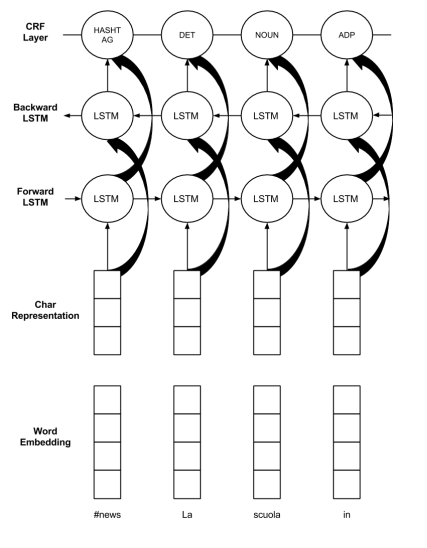
\includegraphics[width=0.28\textwidth]{figure/Architettura1.png}
\captionof{figure}{DL architecture sequence labeling}

\section{Tasks}

In this section, known tasks of the NLP will be dealt with.
The tasks that we will deal with are: Part-of-speech tagging (Pos Tagging), Named-entity recognition (NER), Super-Sense Tagging (SST), other sentiment classification tasks that will be discussed later.\\
In the work done each task is contextualized with a real example. The decrees follow:

\subsection{Pos Tagging of Tweets}

The part of speech explains how a word is used in a sentence.\\
There are eight main parts of speech (nouns, pronouns, adjectives, verbs, adverbs, prepositions, conjunctions and interjections).
POS tagging is a supervised learning solution that uses features like the previous word, next word, is first letter capitalized etc. NLTK has a function to get pos tags and it works after tokenization process.\\
The most popular tag set is Penn Treebank tagset.\\
Most of the already trained taggers for English are trained on this tag set, but in this work is used PoSTWITA. PoSTWITA is a PoS Tagset buil on pourpose in 2016.\\
We apply this task to the world (or tokens) of tweets.\\
The goal of the task is to perform PoS tagging of tweets.\\
The task is more challenging than the classic PoS tagging due to the short and the noisy nature of tweets.\\
For the evaluation we adopt the data set used during EVALITA 2016 PoSTWITA.\\
The data set contains 6,438 tweets (114,967 tokens) for training and 300 tweets (4,759 tokens) for the test.\\
The metric used for evaluation is the classic coding precision: it is defined as the correct assignment number of the PoS tag divided by the total number of tokens in the test set. Participants can only provide one tag for each token. All the best performing PoSTWITA systems are based on deep neural networks and, in particular, on LSTM, moreover, most systems use word or character ads as input to their systems.
It is important to underline that the best system (ILC-CNR) \cite{DBLP:conf/clic-it/CiminoD16}(Cimino and Dell'Orletta, 2016) in PoSTWITA uses a biLSTM and an RNN using
both words and character spells, also uses additional features based on the morpho-syntactic category and spell checker. The good performance of the proposed system probably depends on the CRF layer and on the corpus used to construct the word "embeddings", but we will deal with this later.



\subsection{NER task}
Named Entity Recognition (NER) (also known as entity chunking) is a subtask of the information extraction that seeks to identify and classify named entities in the text into predefined categories such as the names of people, organizations, places, time expressions , quantities, monetary values, percentages, etc.
Most of the research on NER systems has been structured as a block of non-annotated text.\\
And producing in output an annotated block of text that highlights the names of the entities.\\
An example: a person name consisting of a token, a two-token company name and a time expression were detected and classified with the NER.\\
Is taken into account the I-CAB 9 dataset used in the 2009 edition of EVALITA (Manuela Speranza 2009).\\
The I-CAB dataset consists of a set of manually annotated news with four types of entities: GPE (geopolitics), LOC (position), ORG (organization), FOR (person). 
The data set contains 525 news for the training and 180 for the test for a total number of 11,410 entities noted for the training and 4,966 entities for the tests.\\
The format in which we find the dataset it's IOB2.\\
This format has the following standards: the tag B (for "begin") denotes the first token of a Entity named, I (for "inside") is used for all other tokens in a named entity and O (for "outside") is used for all other words. The tags of type Entity are: FOR (for Person), ORG (by organization), GPE (by geopolitical entity) or LOC (by position).\\

%BHOOOOOOOO??
%Word embeddings are constructed, then there will be a more accurate description, taking advantage of the Italian version of Wikipedia.
%Word2vec \cite{DBLP:journals/corr/abs-1301-3781}(Mikolov et al., 2013) is used to create embeddings with a size of 300. For the other parameters, standard values provided by word2vec are used.



\subsection{Super Sense Tagging}

Super-sense tagging (SST) is a Natural Language Processing task that consists of annotating each significant entity in text, like nouns, verbs, adjectives and adverbs, within a general semantic taxonomy defined by the lexicographer classes (called super-senses) .\\
SST can be considered as a half-way task between Named-Entity Recognition (NER) and Word Sense Disambiguation (WSD): it is an extension of NER, since it uses a larger set of semantic categories, and it is an easier and more practical task with respect to WSD, that deals with very specific senses.\\
Task materials A corpus for Super-sense tagging was created from the Italian Syntactic-Semantic Treebank (ISST) by a semi-automatic correction and conversion process, followed by manual revision [LREC 2010]. ISST-SST (about 320,000 tokens) is freely available for the task and for research purposes. It will be used for training and development. The test will be performed on a smaller corpus from the Italian Wikipedia.\\
This concerns the classic approach while in the specific case that is the task taken into consideration:
The dataset is tagged using the IOB2 format as for the NER task and contains about 276,000 tokens for training and about 50,000 for testing.



%\href{https://www.wikibooks.org}{(Wikibooks home)}
The definition of this task was taken from the following address: \url {http://www.evalita.it/2011/tasks/SST}



\subsection{Multi-task Learning}
For address previous tasks there is an architecture that we introduce later.\\
Now we introduce lastone task.\\
The architecture is extended for performing multi-task learning.
The goal is jointly learn PoS-tag, polarity and irony. \\
First of all it is important to underline that PoS-tag is assigned to each token occurring in the sentence. The polarity and the irony are assigned to the whole sentence.\\
Is followed a hard parameter sharing approach in which have some shared layers in the bottom of the network and task-specific layers on the top.
This architecture depends on the particular sentiment analysis task that we want to perform.\\
The goal is  solve four binary classification tasks: Subjectivity (true/false), positive polarity  (true/false), negative polarity (true/false) and irony (true/false).
 subsequently training a classifier for these classes jointly with the PoS-tagging task.\\
 Then we will see in particular how architecture is built to address this task.

  
\section{Representation}
Regarding the representation of the text we use the word embeddings approach revisited with a features engeneering.\\
In the following sections the concept of word embeddings, character embeddings and the revisited approach used in this work will be discussed.



\subsection{Word Embeddings}

They are a distributed representation for text that is perhaps one of the key breakthroughs for the impressive performance of deep learning methods on challenging natural language processing problems.
A word embedding is a learned representation for text where words that have the same meaning have a similar representation.\\
Word embeddings are a class of techniques where individual words are represented as real-valued vectors in a predefined vector space. Each word is mapped to one vector and the vector values are learned in a way that resembles a neural network, and hence the technique is often lumped into the field of deep learning.\\
Key to the approach is the idea of using a dense distributed representation for each word.\\
Each word is represented by a real-valued vector, often tens or hundreds of dimensions. This is contrasted to the thousands or millions of dimensions required for sparse word representations, such as a one-hot encoding.
The distributed representation is learned based on the usage of words. This allows \textit{words that are used in similar ways to result in having similar representations}, naturally capturing their meaning. This can be contrasted with the crisp but fragile representation in a bag of words model where, unless explicitly managed, different words have different representations, regardless of how they are used.
Word embedding methods learn a real-valued vector representation for a predefined fixed sized vocabulary from a corpus of text.
The learning process is either joint with the neural network model on some task, such as document classification, or is an unsupervised process, using document statistics. The most famous are GloVe, Word2vec.
The definition of this approach was taken from the following address: \url{https://machinelearningmastery.com}.



\subsubsection{Word Embeddings on this Work}

The best model uses the publicly available 50-dimension word embeddings released by \cite{DBLP:conf/aaai/BordesWCB11} Collobert
et al. (2011b) 2, which were trained on Wikipedia and the Reuters corpus RCV-1.
Two other sets of unpublished recordings have also been tested, namely the GloVe spells by Stanford 3, spanning 6 billion words from Wikipedia and Web text \cite{DBLP:conf/emnlp/PenningtonSM14}(Pennington et al., 2014) and Google
word2vec embargments 4 formats on 100 billion words from Google News \cite{DBLP:journals/corr/abs-1301-3781}(Mikolov et al., 2013).\\
Furthermore, word-based word embeddings have been found to work better, in fact using the GloVe program (Pennington et al., 2014) publicly available and an internal program.
reimplementation 5 of the word2vec program \cite{DBLP:journals/corr/abs-1301-3781}(Mikolov et al., 2013) to train word embeddings also on the RCV1 dataset of Wikipedia and Reuters.



\subsection{Character Embeddings} 
Xiang and Yann \cite{DBLP:journals/corr/ChiuN15} introduced character embeddings and character CNN, which will be discussed later.\\
In a character embedding model, the vector for a word is constructed from the character.
    Word for grams are shared by words, these models are better than word embedding models for word vocabulary - they can generate an embedding for an word. Word embedding models like word2vec can not be used to treat word atomically.
    Character-embedding models to be better than the word-embedding models for words that occur infrequently since the character word embedding models in contrast suffer from a lack of sufficient training opportunity for infrequent words.


\subsubsection{Character Embeddings on this Work}
It starts by randomizing a search table with values derived from a uniform distribution with interval $[-0,5,0.5]$ to generate an embedding of 25-dimensional characters.
The character set includes everything
unique characters in the \cite{DBLP:journals/corr/cs-CL-0306050}CoNLL-2003 data set 8 plus special tokens
PADDING and CONDITION. The PADDING token is used for the CNN and the UNKNOWN token is used for all other characters (which appear in OntoNotes). For all experiments, the same set of random joints was used.

\subsection{Additional Word-level Features}
In this section are described additional methodologies applied is features engennering.\\
The first apporach it focuses on uppercase information.\\
The uppercase information is deleted during the embedding word search, the Collobert method is evaluated to use a separate search table for add to the capitalization function with the following options: \textit{allcaps, upperInitial, lowercase, mixedCaps, noinfo}.
\cite{DBLP:conf/aaai/BordesWCB11}(Collobert et al., 2011b).\\
The second approach it focuses on lexicon.\\
Most state of the art NER systems make use of lexicons as a form of external knowledge.\\
For   each   of   the   four   categories   (Person, Organization, Location,Misc)  defined  by the CoNLL 2003 NER shared task, is compiled a list  of  known  named  entities  from  DBpedia,  by extracting all descendants of DB-pedia  types  corresponding  to  the  CoNLL  categories.
No separate lexis were built for the OntoNotes (\url{https://catalog.ldc.upenn.edu/LDC2013T19}) tag set because the matches between the DBpedia (\url{https://catalog.ldc.upenn.edu/LDC2013T19}) categories and its tags could not be found in many cases. Furthermore, for each item first removed the brackets and all the text contained inside, then the stripped final punctuation.
For each category of vocabularies, it is match every n-gram (up to the length of the longest vocabulary) with respect to the vocabulary. A game it is successful when the n-gram corresponds to the prefix o suffix of an entry and is at least half the length of the entrance. Because of the high potential of ous matches, for all categories except Person , it is discard partial lots of less than 2 tokens.
When there are multiple overlapping correspondences inside
in the same category, is prefered exact matches compared to test matches, and then shorter longer matches
matches and lastly matches in the sentence over the next games.
All games are insensitive houses.
For each token in the game, the function is coded  in  BIOES annotation.
indicating the position of the token in the matched entry. In other words,B will not appear in a suffix only partial match, and E will not appear in a prefix-only partial match.

\subsection{Additional Character-level Features}
A search table is used to generate a 4-dimensional
vector representing the type of character (superior
case, minuscule, punctuation, other).

The construction of the embeddings was taken by the following source:\url{https://www.aclweb.org/anthology/Q16-1026}.


\vskip 0.5cm

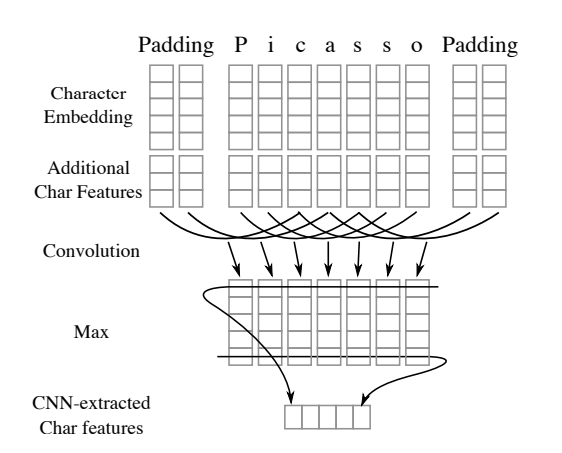
\includegraphics[width=0.38\textwidth]{figure/charEmbb.png}
\captionof{figure}{Character-Embedding lev.}

%%%%%%%%%%%%%%%%%%%%%%%%%%%%%%%%%%%%%%%%%%%%%%%%%%%%%%%%%%%%%%%%%%%%%%
\section{Architecture}

After dealing with the tasks on which we will work, the used architecture will be introduced to the used representation.The architectures used will first be introduced and then their use in the work examined will be contextualised.\\
The architecture is sketched in Fig.1: The input level of the Convolutional Neural Network (CNN) is represented by the character-level representation  of which we have spoken previously. A dropout layer \cite{DBLP:journals/jmlr/SrivastavaHKSS14}(Srivastava et al. 2014) with convolution and max pooling is applied before feeding the CNN with character embeddings. 
Then, the character embeddings are concatenated with the word embeddings to form the input
for the Bi-directional LSTM (bi-LSTM) layer, that we will introduce better later, as sketched in Fig. 2. 
The dropout layer is also applied to output vectors from the LSTM layer. 
The output layer is based on Conditional Random Fields (CRF) and it modifies the output vectors of the LSTM in order to find the best output sequence.
The initial pourpose will always be followed, is treatment of the topics with lexicon easy to understand.

\subsection{CNN}
%extracting character features https://www.aclweb.org/anthology/Q16-1026
In this section we speak of Extracting of Character Features Using a Convolutional Neural Network (CNN).
\subsubsection{What's CNN?}
For an easy description we can star with definition of \textit{\textbf{convolution}}.
The for me easiest way to understand a convolution is by thinking of it as a sliding window function applied to a matrix. The matrix can represent anything: pixels of an image, words, characters.\\
 Each entry of start matrix that corresponds to one pixel, word or character, it can have a value. The sliding window is called a kernel, filter, or feature detector. We use a $n×m$ filter, multiply its values element-wise with the original matrix, then sum them up. To get the full convolution we do this for each element by sliding the filter over the whole matrix. \\
Taking the difference between a pixel, word or character and its neighbors detects information.\\
Now we know what convolutions are.
But what about \textit{CNNs}? CNNs are basically just several layers of convolutions with nonlinear activation functions like ReLU or tanh applied to the results. In a classic feedforward neural network we connect each input neuron to each output neuron in the next layer. That's also called a fully connected layer. In CNNs we do not do that. Instead, we use convolutions over the input layer to compute the output. This results in local connections, where each region of the input is connected to a neuron in the output. Each layer applies different filters, typically hundreds or thousands  and combines their results. There's also something called pooling (subsampling) layers.\\
%POOLING
 \textit{Pooling layers} subsample their input. The most common way to do pooling it to apply a max operation to the result of each filter.
 In NLP we typically are apply pooling over the complete output, yielding just a single number for each filter.
 One property of pooling is that it provides a fixed size output matrix, which typically is required for classification.\\
Pooling also reduces the output dimensionality but (hopefully) keeps the most salient information. You can think of each filter as detecting a specific feature, such as detecting if the sentence contains a negation like “not amazing” for example. If this phrase occurs somewhere in the sentence, the result of applying the filter to that region will yield a large value, but a small value in other regions. By performing the max operation you  are keeping information about whether or not the feature appeared in the sentence, but you are losing information about where exactly it appeared.  


\subsubsection{How in NLP?}

In the case of a NLP tasks: each row of the matrix one token, typically a word or character like our work. Word is a word. Typically, these vectors are word embeddings (low-dimensional representations) like word2vec or GloVe, but they could also be one-hot vectors that index the word into a vocabulary. For a 10 word sentence using a 100-dimensional embedding we would have a $10 × 100$ matrix as our input.
For each word it's employ a convolution and a max layer to extract a new feature vector from the per-character feature vectors such as character embeddings and (optionally) character type.  Words are padded with a number of special PADDING characters on both sides depending on the window size of the CNN.
The hyper-parameters of the CNN are the window size and the output vector size.\\
The input level of the Convolutional Neural Network (CNN) is represented by the character-level representation \cite{DBLP:journals/corr/ChiuN15}(Chiu and Nichols 2015). A dropout layer \cite{DBLP:journals/jmlr/SrivastavaHKSS14}(Srivastava et al. 2014) with convolution and max pooling is applied \cite{DBLP:journals/corr/ChiuN15}(Chiu and Nichols 2015 sec. 1) obtaining a fixed length feature vector from character-level features. This is the feeding of CNN, which as said will return fixed length feature vector.\\
%before feeding the CNN with character embeddings. 
Then, the character embeddings are concatenated with the word embeddings to form the input for the Bi-directional LSTM (bi-LSTM).
Therefore, for each word, these vectors are concatenated and fed to the Bi-LSTM,
which we will talk about later.

\includegraphics[width=0.38\textwidth]{figure/charEmm+CNN.png}
\captionof{figure}{CNN and Bi-LSTM}

\subsection{LSTM}
% https://www.aclweb.org/anthology/Q16-1026 paragrafo 2.2
Long Short Term Memory networks – usually just called \cite{hochreiter1997long}“LSTMs” – are a special kind of RNN, capable of learning long-term dependencies.\\
LSTMs are explicitly designed to avoid the long-term dependency problem. Remembering information for long periods of time is practically their default behavior.\\
LSTMs help preserve the error that can be backpropagated through time and layers. By maintaining a more constant error, they allow recurrent nets to continue to learn over many time steps (over 1000), thereby opening a channel to link causes and effects remotely.
LSTMs contain information outside the normal flow of the recurrent network in a gated cell. Information can be stored in, written to, or read from a cell. The cell makes decisions about what to store, and when to allow reads, writes and erasures, via gates that open and close.\\
\textbf{Memory Cell?} This is a special neuron for memorizing long-term dependencies. LSTM contains an internal state variable which is passed from one cell to the other and modified by Operation Gates.\\
LSTM is smart enough to determine how long to hold onto old information, when to remember and forget, and how to make connections between old memory with the new input. \\
This is a brief description of what an LSTM is, the architecture taken into consideration uses a Bi-LSTM.\\

\subsection{Bi-LSTM}
% vedi qui https://towardsdatascience.com/introduction-to-sequence-models-rnn-bidirectional-rnn-lstm-gru-73927ec9df15
For this work a veriante of LSTM was used, it is called Bi-LSTM.
In this section the Bi-LSTM is introduced and a general description is made and in the second part 
the application in this work is treated.\\

\subsubsection{What's Bi-LSTM?}

Bi-LSTM is variety of neural network based models. These models include LSTM networks, bidirectional
LSTM networks (BI-LSTM). In sequence tagging task, we have access to both past and future input features for a given time, we can thus utilize a bidirectional LSTM network as proposed in \cite{DBLP:journals/corr/Graves13}(Graves et al., 2013). 
In doing so, we can efficiently make use of past features (via forward states) and future features (via backward states) for a specific time frame. We train bidirectional LSTM networks using backpropagation
through time (BPTT).
The forward and backward passes over the unfolded network over time are carried out in a similar
way to regular network forward and backward passes, except that we need to unfold the hidden states for all time steps. We also need a special treatment at the beginning and the end of the data points.
\subsubsection{How in this work?}
After having taken in feeding concatenated vectors (see previous section).
There is a split:
\begin{itemize}
\item The output vectors are fed to a second Bi-LSTM level. 
\item The output vectors are fed to CRF level.
\end{itemize}
In this section we only deal with the second level of Bi-LSTM.\\
The dropout layer is also applied to output vectors from the second Bi-LSTM layer. 
This new layer based on a bi-LSTM is added using the same dimension of the first LSTM layer.
Then, a dropout layer is applied and the final classes probabilities are computed by a binary
cross entropy function for each class.
In this case the last layer does not predict a tag for each token, but it predicts only one tag 5 for each classification task (subjectivity, positive, negative, irony). 
%The multi-task architecture is sketched in Figure 3.
Moreover, as we have already mentioned, the output of the first bi-LSTM layer is the input of the CRF layer to predict PoS tags, while each binary feeling activity is implemented by a new one
LSTM level and cross-entropy function.

\vskip 0.5cm
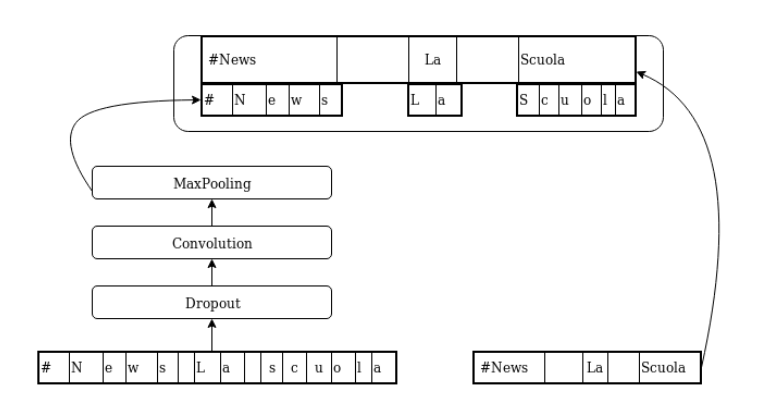
\includegraphics[width=0.38\textwidth]{figure/2.png}
\captionof{figure}{Input level of DL Architecture }
\vskip 1.5cm



\subsection{CRF}
%https://arxiv.org/pdf/1508.01991.pdf
There is way to make use of neighbor tag information in predicting current tags. it's focus on sentence level instead of individual positions, thus leading to Conditional Random Fields (CRF) models \cite{Lafferty01conditionalrandom}(Lafferty et al., 2001) . Note that the inputs and outputs are directly connected, as opposed to LSTM and bidirectional LSTM networks where memory cells/recurrent components are employed.
It has been shown that CRFs can produce higher tagging accuracy in general.
\subsubsection{How we use?}
We use the CRF level, parallel to the second Bi-LSTM level, for predicting PoS-tags. 
This level will feed the aforementioned vectors and provide predictions as output.

\subsubsection{Why use?}
Using output layer that is based on Conditional Random Fields (CRF) it modifies the output vectors of the LSTM in order to find the best output sequence. The CRF layer is useful for learning correlations between labels in neighborhoods.

\vskip 1cm

\subsection{Multi-task learning}

Previously we had talked about the existence of two parallel models located on the second level.
CRF has been addressed previously.Now we focus on the second bi-LSTM.\\
As already mentioned, the dropout layer is also applied to output vectors from the second Bi-LSTM layer. 
This new layer based on a bi-LSTM is added using the same dimension of the first LSTM layer.
Then, a dropout layer is applied and the final classes probabilities are computed by a binary
cross entropy function for each class.In this case the last layer does not predict a tag for each token, but it predicts only one tag 5 for each classification task (subjectivity, positive, negative, irony). 

\vskip 0.5cm

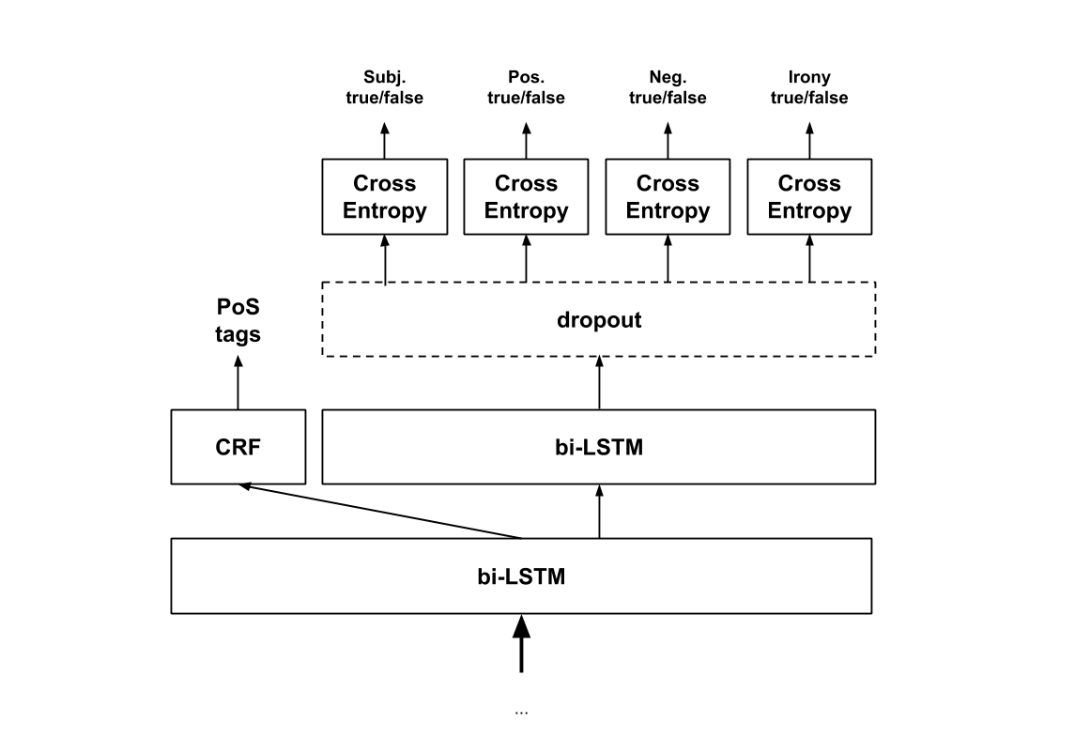
\includegraphics[width=0.52\textwidth]{figure/Architettura2.png}
\captionof{figure}{DL architecture for multi-task learning.}
 
%%%%%%%%%%%%%%%%%%%%%%%%%%%%%%%%%%%%%%%%%%%%%%%%%%%%%%%%%%%%%%%%%%%%%%
\section{Datasets}
In this section we take care of the data that have been used to train or test the architecture.
We want to emphasize that many tasks are performed using Italian datasets.\\
In particular we exploit data coming from the last edition (2016) of EVALITA\url{https://github.com/evalita2016/data} and the previous ones EVALITA \url{https://github.com/evalita2011} is a periodic evaluation campaign of NLP and speech tools for the Italian language.\\
Other datasets are instead of common domain.

\subsection{Dataset for Pos-Tagging}
For the evaluation we adopt the dataset used during EVALITA 2016.
The dataset contains 6,438 tweets (114,967 tokens) for training and 300 tweets (4,759 tokens) for testing.

\vskip 0.5cm
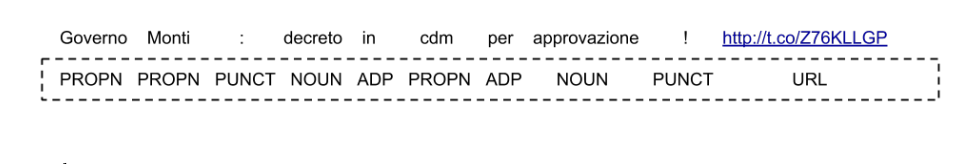
\includegraphics[width=0.42\textwidth]{figure/postexample.png}
\vskip 0.5cm

The only used resource is a corpus of 70M tweets randomly extracted from Twita, a collection of about 800M tweets, for building the word embeddings.

\vskip 1cm

\subsection{Dataset for NER}
For NER task is used I-CAB dataset. The I-CAB dataset consists of a set of news manually annotated
with four kinds of entities: GPE (geo-political), LOC (location), ORG (organization) and
PER (person). The dataset contains 525 news for training and 180 for testing for a total
number of 11,410 annotated entities for training and 4,966 ones for testing. The dataset
is provided in the IOB2 format: the tag B (for “begin”) denotes the first token of a
Named Entity, I (for “inside”) is used for all other tokens in a Named Entity, and O
(for “outside”) is used for all other words. The Entity type tags are: PER (for Person),
ORG (for Organization), GPE (for GeoPolitical Entity), or LOC (for Location). \\
Next image is an example of the output of the NER task.\\
We can see that each token has been labeled with the IOB2 and I-CAB format.\\
\vskip 0.5cm
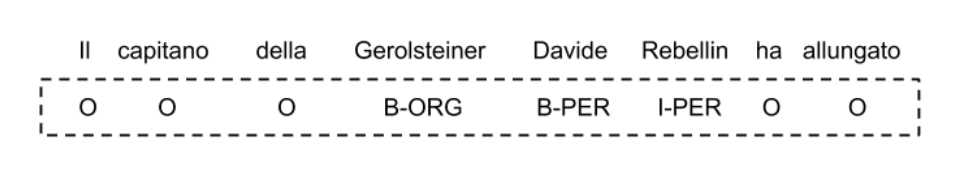
\includegraphics[width=0.44\textwidth]{figure/nerexample.png}
\vskip0.5cm


\subsection{Dataset for Super Sense Tagging}
The dataset has been tagged using the IOB2 format as for the NER task and contains about 276,000 tokens for training and about 50,000 for testing. In training each token occurring in WordNet is annotated
with its super sense.

\vskip 0.5cm
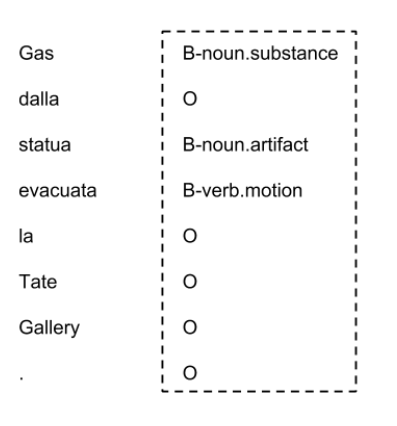
\includegraphics[width=0.32\textwidth]{figure/sstexample.png}
\vskip0.5cm

\subsection{Dataset for Word Embeddings}
The building of word embeddings by exploiting the Italian version of Wikipedia.
Word2vec \cite{DBLP:journals/corr/abs-1301-3781}(Mikolov et al. 2013) is used for creating embeddings with a dimension of 300; removing all words that have less than 40 occurrences in Wikipedia. For the other parameters, is adopted the standard values provided by word2vec.

\subsection{Dataset for Multi-task Evaluation}
Sentiment data are taken from SENTIPOLC.
SENTIPOC (SENTIment POLarity Classification) is a sentiment analysis task where systems are required to automatically annotate tweets with a tuple of boolean values indicating the message’s subjectivity, its polarity (positive or negative), and whether it is ironic or not.
The SENTIPOLC training set consists of 7,410 tweets (6,412 are shared with the
PoSTWITA task), while the test set contains 2,000 tweets (300 are shared with PoST-WITA).



%%%%%%%%%%%%%%%%%%%%%%%%%%%%%%%%%%%%%%%%%%%%%%%%%%%%%%%%%%%%%%%%%%%%%%
\section{Parameters}

In this section the architectural parameters will be described. It is also important to note that in the past was already proposed an evaluation on these tasks \cite{DBLP:conf/clic-it/BasileSC17}(Basile, Semeraro, and Cassotti 2017) using the same architecture, but without correctly optimizing hyperparameters due to the lack of a validation set. In this paper, second version, is described a procedure for hyperparameters optimization based on k-fold cross-validation.\\
Furthermore, together with the parameters and the results obtained in each task, results of systems that approach the same tasks in different ways will also be shown.\\
We start talking about the Bi-LSTM and then move on to the individual cases.In the following subsections follow a more detailed description.

\subsection{Parameters of Bi-LSTM}

\vskip 0.5cm
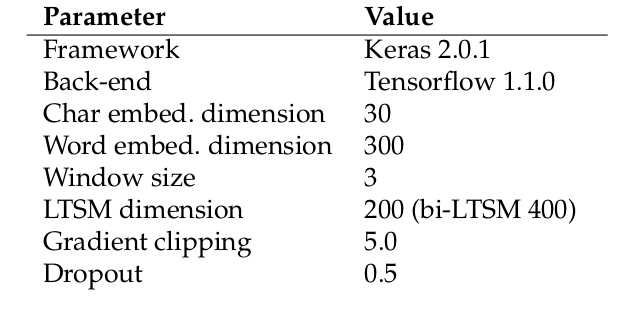
\includegraphics[width=0.38\textwidth]{figure/paramBiLSTM.png}
\captionof{figure}{This is a param of Bi-LSTM. }
\vskip0.5cm
The perform parameters optimization using 5-fold cross-validation on training data since EVALITA does not provide a validation set. In particular, is perform optimization in order to choose the best optimization algorithm evaluating among Adadelta, Adagrad, Adam and SGD. 
Regarding SGD, is test several values of the initial learning rate in the set ${[0.01, 0.0125, 0.15]}$ and values for the decay rate in the set ${[0.01, 0.05, 0.1]}$.
Moreover, optimize the number of epochs (setting the maximum number of epochs to 60).
Results of the optimization procedure are reported in next table. Results about SGD parameters are removed since they give rise to lower performance.
\vskip 0.5cm
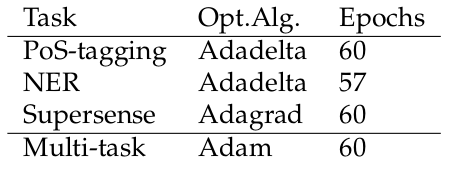
\includegraphics[width=0.38\textwidth]{figure/resultBiLSTMOPT.png}
\captionof{figure}{This is a result of Bi-LSTM optimization. }
\vskip0.5cm



\subsection{Parameters \& Results on Pos-Tag }
 In \cite{DBLP:conf/clic-it/BasileSC17}(Basile, Semeraro and Cassotti 2017), we have same architecture and different parameters.\\
 Accuracy reported of \textit{.9334} using the same system, but running more epochs (100 epochs).\\
 In this work, the maximum number of epochs to 60 during the optimization step in order to reduce the computation time. 
 Nevertheless, results prove the effectiveness of the proposed architecture without exploiting task/language specific resources. The only used resource is a corpus of 70M tweets randomly extracted from Twita, a collection of about 800M tweets, for building the word embeddings.

\vskip 0.5cm
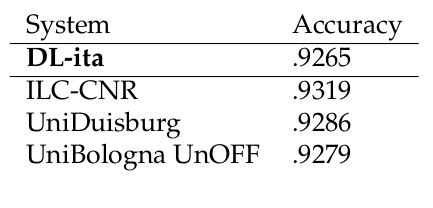
\includegraphics[width=0.38\textwidth]{figure/posttask.png}
\captionof{figure}{There are a results of Pos-Tagging of of some recent works PoSTWITA. }
\vskip0.5cm


\subsection{Parameters \& Results on NER}
For the official evaluation of system results the organizers of evalita 2009 used the scorer made available
by CONLL for the 2002 Shared Task, which can be freely downloaded from the
CONLL website.\\
With respect to the results submitted by the participants (each participant was allowed to submit up to two runs), the CONLL scorer computes the following evaluation measures: Precision, Recall, and F-Measure (FB1).\\
Precision indicates the percentage of correct positive predictions and is computed as the ratio between the number of Named Entities correctly identified by the system (True Positive) and the total number of Named Entities identified by the system (True
Positive plus False Positive).
Precision = TP / (TP + FP)\\
Recall indicates the percentage of positive cases recognized by the system and is computed as the ratio between the number of Named Entities correctly identified by the system (True Positive) and the number of Named Entities that the system was
expected to recognize (True Positive plus False Negative).Recall = TP / (TP + FN)\\
F-Measure, the weighted harmonic mean of Precision and Recall computed as has been used for the official ranking.
FB1= 2 (Precision  Recall) / (Precision + Recall)\\
In next Table, where the system (DL-ita) is compared with respect to the other EVALITA 2009 participants.\\
The system outperforms the first three EVALITA participants thanks to the best performance in recall.\\
All the first three participants adopt classical classification methods: the first system combines two classifiers (HMM and CRF), the second participant uses a Perceptron algorithm, while the third partecipant adopts Support Vector Machine and feature selection.\\
We can conclude that the DL architecture is more effective in model generalization and in tackling the data sparsity problem. This behavior is supported by the good performance in recognizing LOC entities.
In fact, the LOC class represents about the 3\% of annotated entities in both training and test.
Other two systems able to overcome the EVALITA 2009 participants have been proposed in the
literature. 
The former (Nguyen and Moschitti 2012) achieves the 84.33\% of F1 by using re-ranking techniques and the combination of two state of the art NER learning algorithms: conditional random fields and support vector machines. 
The latter exploits a Deep Neural Network with a log-likelihood cost function and a recurrent feedback mechanism to ensure the dependencies between the output tags. This system is able to achieve the 82.81\% of F1, a performance comparable with our DL architecture.
This is what the article says that I am considering \cite{DBLP:conf/clic-it/BasileSC17}.

\vskip 0.5cm
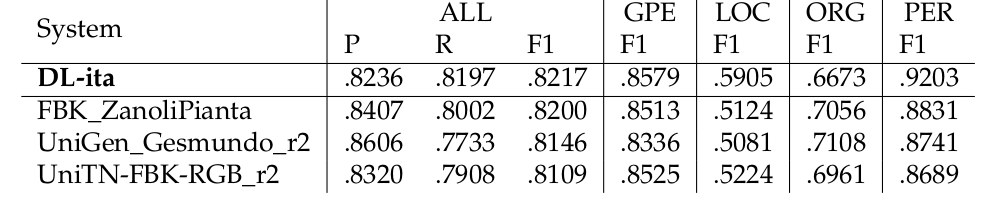
\includegraphics[width=0.52\textwidth]{figure/nerresult.png}
%\captionof{figure}{?????????????????????? }
\vskip0.5cm

\subsection{Parameters \& Results on SS Tagging}
The dataset, like descrciption in previous section, has been tagged using the IOB2 format as for the NER task and contains about 276,000 tokens for training and about 50,000 for testing. A training
sample each token occurring in WordNet is annotated with its super sense. The metric adopted for the evaluation is the F1. Results of the evaluation are reported in next Table.

\vskip 0.5cm
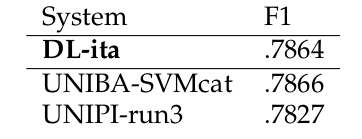
\includegraphics[width=0.28\textwidth]{figure/sstresult.png}
%\captionof{figure}{?????????????????????? }
\vskip0.5cm

As word embeddings, is used the same ones adopted for the NER task and built upon Wikipedia with lowercase. Moreover, is exploited PoS-tags as additional features.\\
The system (DL-ita) is very close to the best system in EVALITA 2011 SST task UNIBA-SVMcat. 
This system combines lexical and distributional features through an SVM classifier, in particular it exploits specific features such us: lemma, contextual PoS-tags, the super-sense assigned to the most frequent sense of the word and information about the grammatical conjugation of verbs. We plan to introduce this kind of features into the DL system in order to understand if this difference in performance still emerges.
The second system (UNIPI-run3) exploits lexical features and a Maximum Entropy classifier.\\
This is what the article says that I am considering \cite{DBLP:conf/clic-it/BasileSC17}.


\subsection{Parameters \& Results on Multi-task Evaluation}

As already mentioned in the previous section sentiment data are taken from
SENTIPOLC. SENTIPOC (SENTIment POLarity Classification) is a sentiment analysis task where systems are required to automatically annotate tweets with a tuple of boolean values indicating the message’s subjectivity, its polarity (positive or negative), and whether it is ironic or not.
Without dwelling on the characteristics of SENTIPOLC, already dealt with.
 The traininig of multi-task architecture use 6,412 tweets, while the accuracy of PoS-tag is evaluated on 300 tweets and the performance on SENTIPOLC is computed on 2,000 tweets.\\
 
\vskip 0.5cm
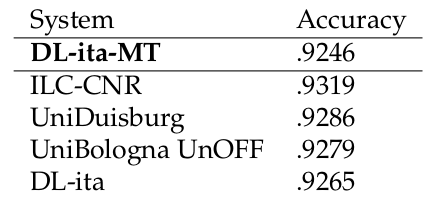
\includegraphics[width=0.28\textwidth]{figure/Multiresult.png}
\captionof{figure}{This is result of challenge PoSTWITA task using the multi-task architecture}
\vskip0.5cm


But beware as the results show that the PoS tag is not able to exploit the information on polarity and irony to improve performance.\\


In the next table we can see the results of SENTIPOLC task.\\
Evaluation of SENTIPOLC task, systems are evaluated on the assignment of a 0 or 1 value to the subjectivity field. A response is considered plainly correct or wrong when compared to the gold standard annotation.\\
The same speech was made for the irony task.\\
For polarity classification: the coding system allows for four combinations of opos and oneg values: 10 (positive polarity), 01 (negative polarity), 11 (mixed polarity), 00 (no polarity).\\
Accordingly, we evaluate positive and negative polarity independently by computing precision, recall and F-score for both classes (0 and 1). The F-score for the two polarity classes is the average of the F-scores of the respective pairs.
Finally, the overall F-score for second subtask is given by the average of the F-scores of the two polarities.\\
Regarding the SENTIPOLC task, results show that the multi-task architecture is able to improve its performance in the irony task. 

\vskip 1.5cm
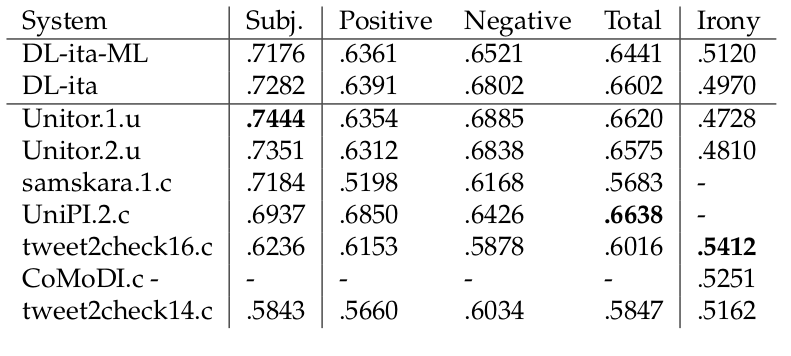
\includegraphics[width=0.48\textwidth]{figure/sentipolc.png}
\captionof{figure}{Results for the SENTIPOLC task}
\vskip 1cm

We can see that the performance decreases in the polarity task in fact, the values are around $0.6$ .\\
In conclusion, information about the PoS-tag is useful for irony, but not in the subjective and polarity tasks.\\
It is not easy to interpret the DL architecture and this is made even more difficult by the multi-task learning.\\
Also , are reports results for the systems at the intersection between the first three systems of each SENTIPOLC subtask. The system (DL-ita-ML) is able to achieve good results in each subtask and ranks 4 out of 18 in the subjective task, 6 out of 25 in the polarity task and 5 out of 12 in the irony task.
The best system in the subjective task, Unitor1.u \cite{DBLP:conf/acl/CroceFCB17}(Castellucci, Croce, and Basili 2016), reports also good performance in the polarity task but poor performance in the irony task.\\
The best system in the polarity task, UniPI.2, adopts Convolutional Neural Networks as Unitor1.u and exploits both word embeddings and Sentiment
Specific word embeddings.\\
This system ranks eighth in the subjective task and does not participate in the irony one.\\
Finally, the best system in the irony task, tweet2check16.c, is an industrial system which combines many different classifiers, each of which is built by using different machine learning algorithms and implementing different features.\\
In conclusion, the multi-task architecture obtains good performance in all Sentiment Polarity Classification subtasks.\\
However, it does not achieve the best performance in any specific task. Moreover, we observe that the information about PoS-tags is useful in the irony subtask, while the use of polarity information in the PoS-tag results in a slight decrease in accuracy.
%%%%%%%%%%%%%%%%%%%%%%%%%%%%%%%%%%%%%%%%%%%%%%%%%%%%%%%%%%%%%%%%%%%%%%


%%%%%%%%%%%%%%%%%%%%%%%%%%%%%%%%%%%%%%%%%%%%%%%%%%%%%%%%%%%%%%%%%%%%%%
%\section{Results}

%\footnotetext{Examine the input file, asme2ej.tex, to see how a footnote is given in a head.}

%Footnotes are referenced with superscript numerals and are numbered consecutively from 1 to the end of the paper\footnote{Avoid footnotes if at all possible.}. Footnotes should appear at the bottom of the column in which they are referenced.


%%%%%%%%%%%%%%%%%%%%%%%%%%%%%%%%%%%%%%%%%%%%%%%%%%%%%%%%%%%%%%%%%%%%%%
\section{Conclusion}
In this paper is proposed a easy review of an evaluation of a state of the art DL architecture in the context of language in specific Italian considering some sequence labeling task.\\
In particular, are considered three sequence labeling tasks: PoS-tagging of tweets, Named Entity Recognition and Super-Sense Tagging  and a multi-task learning architecture involving PoS-tagging and sentiment analysis. 
All tasks exploit data coming from EVALITA. \url{http://www.evalita.it}.\\
This system is able to achieve good performance in all the tasks without using hand crafted features. \\
 
Analyzing the results of this system and other systems generally system porposed in EVALITA competitions.\\
 For each tasks we observe that the system is able to achieve state of the art performance for the Italian language in all the sequence labeling tasks.\\
This proves the effectiveness of the DL architecture in a different language in this case Italian - without using language specific features.\\
Instead, many systems with which the comparison was made use massively language specific features.

While the multi-task learning, this architecture is able to achieve good performance in each subtask (subjectivity, polarity and irony) using the same architecture.

In addition, we can observe, the multi-task learning results show that the irony task benefits from the information provided by PoS-tags. \\


Furthermore, we need to underline the winning choice of the authors \cite{DBLP:conf/clic-it/BasileSC172} of this work as regards the construction of the input.\\
Because most word embedding methods take a word as a basic unit and learn embeddings according to words’ external contexts, ignoring the internal structures of words.\\
However, in some languages such as Italian or Chinese, a word is usually composed of several characters and contains rich internal information.\\
The semantic meaning of a word is also related to the meanings of its composing characters.\\
Instead in this work a double level input was used as previously described.\\
This added to the DL architecture provides good performance.






%%%%%%%%%%%%%%%%%%%%%%%%%%%%%%%%%%%%%%%%%%%%%%%%%%%%%%%%%%%%%%%%%%%%%%



%%%%%%%%%%%%%%%%%%%%%%%%%%%%%%%%%%%%%%%%%%%%%%%%%%%%%%%%%%%%%%%%%%%%%%
% The bibliography is stored in an external database file
% in the BibTeX format (file_name.bib).  The bibliography is
% created by the following command and it will appear in this
% position in the document. You may, of course, create your
% own bibliography by using thebibliography environment as in
%
% \begin{thebibliography}{12}
% ...
% \bibitem{itemreference} D. E. Knudsen.
% {\em 1966 World Bnus Almanac.}
% {Permafrost Press, Novosibirsk.}
% ...
% \end{thebibliography}

% Here's where you specify the bibliography style file.
% The full file name for the bibliography style file 
% used for an ASME paper is asmems4.bst.
\bibliographystyle{wmrDoc}

% Here's where you specify the bibliography database file.
% The full file name of the bibliography database for this
% article is asme2e.bib. The name for your database is up
% to you.

\newpage

\bibliography{wmrDoc}


\end{document}
